\section{Symmetric Matrices}
%Lecture Sep 18
The set of $n$ by $n$ square matrix is defined as
$$S^n = \{A\in \reals^{n\times n} | A = A^T \}$$

\vspace{0.3cm}
Following are a few examples of symmetric matrix

Example 1: Hessian matrix: A matrix that each element is the 2nd order partial derivative of $F$
$$[\nabla^2 F]_{ij} = \frac{\sigma}{\sigma x_i}\frac{\sigma}{\sigma x_j}F(x)$$

Example 2: Quadratic Functions: $q: \reals^n \rightarrow \reals$
\begin{align*}
q(x) &= \sum^n_{i=1}\sum^n_{j=1}a_{ij}x_ix_j + \sum^n_{i=1}c_ix_i + d\\
&= x^TAx + c^Tx + d\\
&= \frac{1}{2}x^T(A + A^T)x + c^Tx + d\\
&= \frac{1}{2}
\begin{bmatrix}%
x^T& 1
\end{bmatrix}
\begin{bmatrix}%
A + A^T & C\\
C^T & 2d
\end{bmatrix}
\begin{bmatrix}%
x\\
1
\end{bmatrix}
\end{align*}


1) Let $F(x) = C^Tx = \sum^n_{i=1}c_ix_i$:
\begin{align*}
\frac{d}{dx_k}F(x) &= \frac{d}{dx_k}(\sum^n_{i=1}c_ix_i) = c_k\\
\nabla F(x) &= 
\begin{bmatrix}%
\frac{\sigma F(x)}{\sigma x_1}\\
...\\
\frac{\sigma F(x)}{\sigma x_n}
\end{bmatrix}=
\begin{bmatrix}%
c_1\\
...\\
c_n
\end{bmatrix} = C
\end{align*}

2) Let
\begin{align*}
F(x) &= x^TAx = \sum_i\sum_ja_{ij}x_ix_j\\
&= a_{11}x_1^2 + a_{12}x_1x_2 + ... + a_{21}x_2x_1 + ...\\
\frac{d}{dx_k}F(x) &= \frac{d}{dx_k}(a_{kk}k_k^2 + \sum_{l\neq k}k_lx_k(a_{kk}+a_{kl}))\\
&= (a_{kk} + a_{kk})x_k + \sum_{l\neq k}x_l(a_{lk} + a_{kl}) \\
&= \sum^n_{i=1}(a_{lk} + a_{kl})x_l\\
&= \sum^n_{i=1}([A]_{kl} + [A]_{lk})x_l
\end{align*}

Hence,
\begin{align*}
\nabla F(x) &= (A + A^T)x\\
[\nabla^2F(x)]_{kj} &= \frac{d}{dx_j}(\frac{\partial}{\partial x_k}F(x))\\
&= [A]_{kj} + [A]_{jk}\\
\nabla^2F(x) &= (A + A^T)
\end{align*}

Combine (1) and (2), and because $q(x) = x^TAx + c^Tx + d$, we take Taylor approximation of $q(x)$ up to the second order:
\begin{align*}
\tilde{q}(x) &= q(0) + \nabla q(0)^Tx + \frac{1}{2}x^T\nabla^2q(0)x\\
&= d + c^Tx + \frac{1}{2}x^T(A + A^T)x
\end{align*}

\subsection{Symmetric Matrices and Eigenvectors}

\begin{theorem}{4.18 \& 4.2 in textbook}
	
	For any matrix in $S^n = \{A\in \reals^{n\times n} | A = A^T \}$:
	
	1) All eigenvalues are purely real(so eigenvectors can be picked purely real).
	
	2) $GM(\lambda_i) = AM(\lambda_i)$: Symmetric matrix is always diagonalizable.
	
	3) Eigenvectors of distinct eigenvalues are $\perp$, i.e.,
	
\qquad $\xi_{\lambda_i} = N(A - \lambda_iI)\perp \xi_{\lambda_i} = N(A - \lambda_jI)$, where $\xi_{\lambda_i}$ denotes the eigenspace w.r.t eigenvalue $\lambda_i$ (also, it is the null space of matrix $(A - \lambda_iI)$).
\end{theorem}

Implication: We can pick the basis for each eigenspace to be an orthogonal basis(e.g, pick the eigenvectors of this symmetric matrix), because we have "Fullset" of eigenvectors($n$ linearly independent vectors) and we can always write:

"Spectral Decomposition":

\begin{align*}
A &= U\Lambda U^{-1}\\
&= U\Lambda U^{T}\\
&= 
\begin{bmatrix}
u^{(1)} & u^{(2)} & \cdots & u^{(n)}\\
\end{bmatrix}
\begin{bmatrix}
\lambda_1 & 0 & 0\\
0 & \ddots & 0\\
0 & 0 & \lambda_n
\end{bmatrix}
\begin{bmatrix}
u^{(1)^T}\\
\vdots\\
u^{(n)^T}
\end{bmatrix}\\
&= \sum^n_{i=1}\lambda_iU^{(i)}U^{(i)^T}
\end{align*}

We summarize our result now: An $n$ by $n$ matrix $A$ is diagonalizable iff there are $n$ linearly independent eigenvectors(subject to scaling factors). In addition, Furthermore, if $A$ is diagonalizable, that is, $A = U\Lambda U^{-1}$, where $\Lambda$ is diagonal matrix with all its entries are the eigenvalues and $U$ is a collection of all its eigenvectors. 

\subsection{Variational Characterization of eigenvalues of $\lambda_i$ where $A\in S^n$} 

We arrange the eigenvalues in a decreasing order, i.e., 
$$\lambda_{max}(A) = \lambda_1 \geq \lambda_2 \geq ... \geq \lambda_n =\lambda_{min}(A)$$


We define the "Rayleigh quotient" as $\frac{x^TAx}{x^Tx}$ for $x\neq 0$, and we propose a theorem for this ratio as follows

\begin{theorem}
For $A\in S^n$, we have 
$$\lambda_{min}(A) \leq \frac{x^TAx}{||x||^2}\leq \lambda_{max}(A),\ \forall x \neq 0$$
\end{theorem}


\begin{proof}
	\begin{align*}
	x^TAx &= x^TU\Lambda U^Tx\\
	&= \bar{x}^T\Lambda\bar{x}\\
	&= \sum^n_{i=1}(\bar{x}_i)^2\lambda_i\\
	&\leq \sum^n_{i=1}(\bar{x}_i)^2\lambda_{max}(A)\\
	&= ||\bar{x}||^2\lambda_{max}(A)
	\end{align*}
where $\bar{x}=U^Tx$, and note that $\Vert \bar{x}\Vert = \Vert {x}\Vert$ since $U$ is orthogonal. Use similar trick we could obtain the lower bound for $x^TAx$. By a simple rearrangement we yield the desired result
	\begin{equation*}
	\lambda(A)_{min}||\bar{x}||^2 \leq x^TAx \leq ||\bar{x}||^2\lambda_{max}(A)
	\end{equation*}
	
	\begin{equation*}
	\lambda(A)_{min} \leq \frac{x^TAx}{||\bar{x}||^2} \leq \lambda_{max}(A)
	\end{equation*}
\end{proof}


\subsection{Positive (Semi) Definite matrices(PD \& PSD)  }

\begin{definition}
	A symmetric matrix $A\in S^n$ is PD (or PSD) if $x^TAx > 0$, $\forall x\in \reals^n$(or $x^TAx\geq 0$).
\end{definition}

Alternatively, we denote the set of PSD matrix and the set of PD matrix as

PSD: $S^n_{+} = \{A\in S^n | A\succeq 0\}$

PD: $S^n_{++} = \{A\in S^n | A\succ 0\}$

Note: The curled inequality symbol $\succeq$ (and its strict form $\succ$) is used to denote generalized inequality: between vectors, it represents component-wise inequality; between matrices, it represents matrix inequality.

\vspace{0.3cm}
Necessary and sufficient conditions:

(1) A symmetric matrix is PSD iff all its eigenvalues $\geq 0$, or, all its \textbf{principal minors} are nonnegative.

(2) A symmetric matrix is PD iff all its eigenvalues $> 0$, or, all its \textbf{leading principal minors} are positive (Sylvester's criterion).

\vspace{0.3cm}
Now we prove the argument for PD:

First, assume $A\in S^n$ is PD, we will show that all $\lambda_i > 0$. 

\begin{equation*}
x^TAx = x^TU\Lambda U^Tx = \bar{x}^T\Lambda\bar{x} = \sum^n_{i=1}\lambda_i(\bar{x}_i)^2 >0
\end{equation*}
Since $A$ is PD and $x\neq 0$, and it is always diagonalizable for a symmetric matrix.

To show this implies $\lambda_j \geq 0, \forall j\in [n]$, we set:
$$\bar{x} = e_j = 
\left[
\begin{matrix}
0\\
0\\
...\\
1\\
0\\
0\\
...
\end{matrix}
\right]
$$
where only the $j$th entry is 1.
$$0 \leq U^{(i)^T} U\Lambda U^TU^{(1)} =e_j^T\Lambda e_j = \lambda_j$$

And now we Assume all eigenvalues are positive, and we want to show that $A$ is PD:
$$x^TAx =x^TU\Lambda U^Tx = \bar{x}^T\Lambda \bar{x} = \sum^n_{i=1}(\bar{x}_i)^2\lambda_i \geq 0$$
The proof is completed.

Recall some previous results and note that:

(1) $\det(A) = \prod^n_{i=1}\lambda_i$

(2) $\det(A) = 0$ iff there exist eigenvalue $\lambda_i = 0$:

(3) Combine (1) and (2) and our proof above, we have
\\ \qquad $\rightarrow$ PD matrices are invertible
\\ \qquad $\rightarrow$ PSD matrices are invertible only if PD





\subsection{Ellipses} 

An ellipse can be defined geometrically as a set or locus of points in the Euclidean plane. Let's consider the following set(an ellipse)
$$
\xi = \{x\in \reals^n | (x - x^{(0)})^T P(x - x^{(0)}) \leq 1 \}
$$
where $P$ is PD.

\begin{marginfigure}
	\centering
	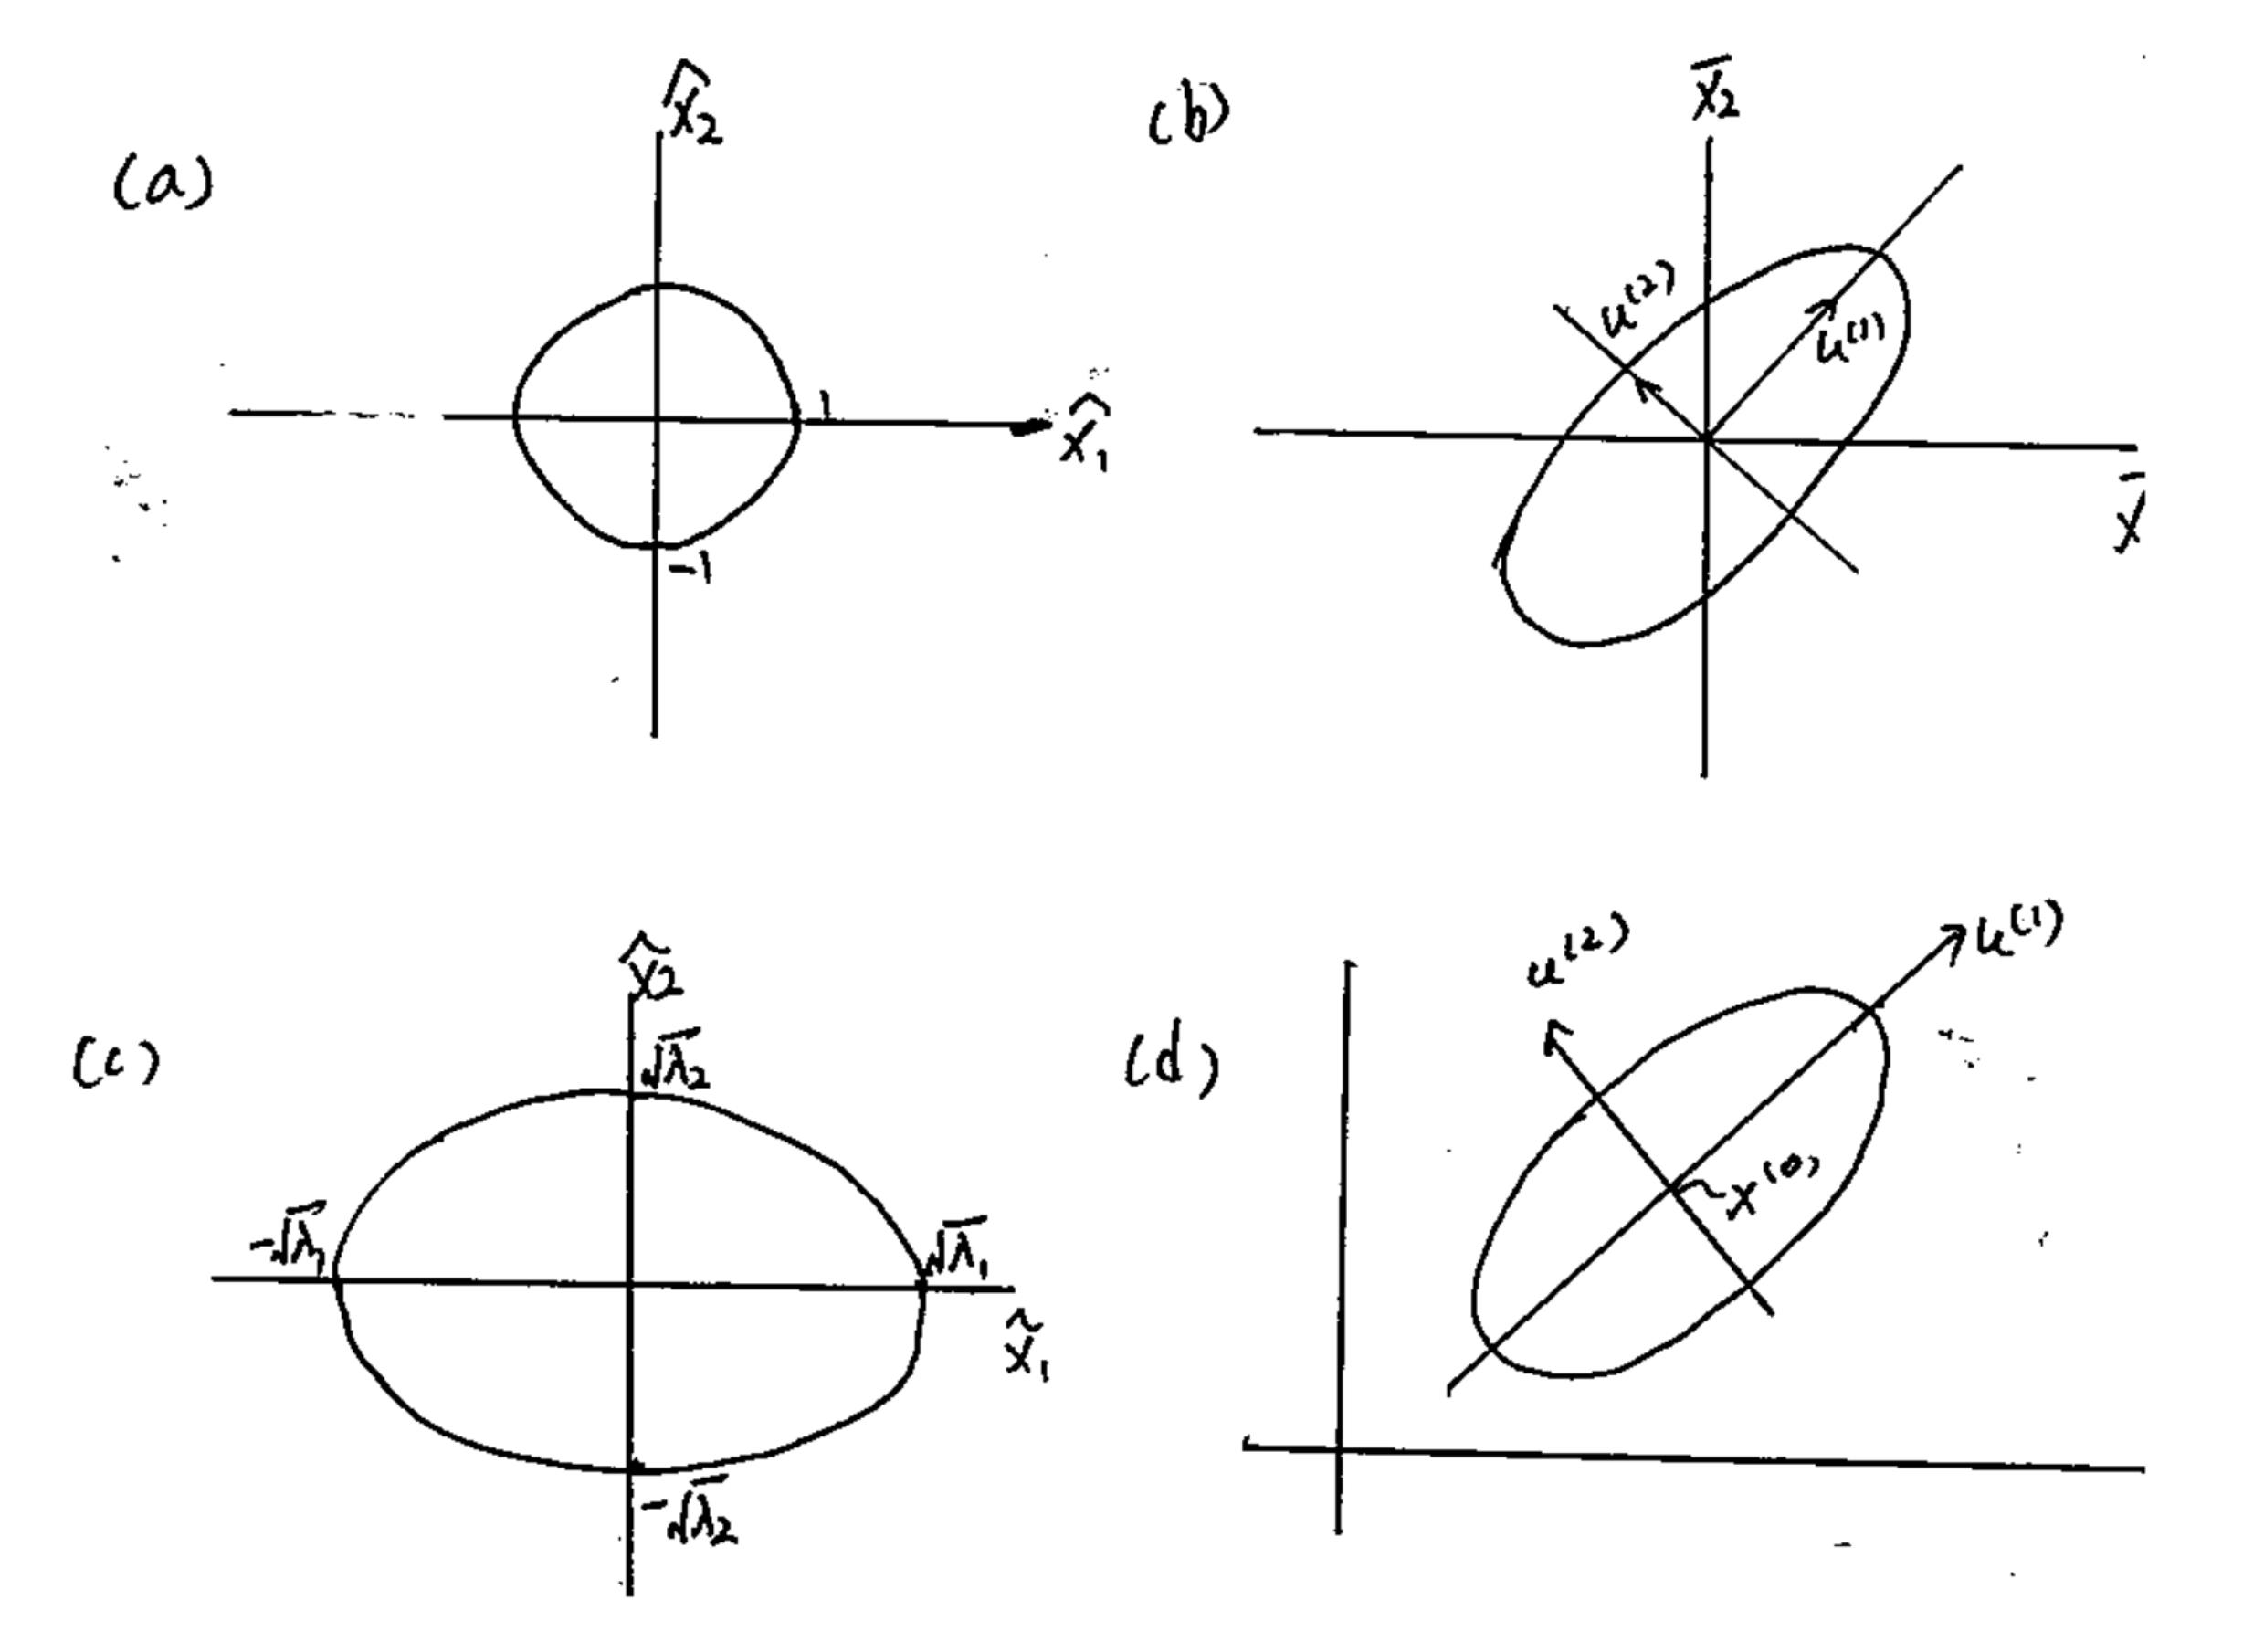
\includegraphics[width=2.1in,height=2.1in]{figures/ch03/figure2.jpg}
	%\caption{This is an inserted JPG graphic} 
	%\label{fig:graph} 
\end{marginfigure}

Note that the argument above is a quadratic function:
\begin{align*}
(x - x^{(0)})^TP^{-1}(x - x^{(0)}) &= x^TP^{-1}x - 2x^{(0)^T}P^{-1}x + x^{(0)^T}P^{-1}x^{(0)}\\
&= x^TAx + c^Tx + d
\end{align*}

Let's look at the set $\xi$, clearly it is centered at $x = x^{(0)}$, and we further simplify it by defining $\bar{x}=x-x^{(0)}$
\begin{align*}
1 &\geq (x - x^{(0)})^TP^{-1}(x - x^{(0)})\\
&= \bar{x}^TP^{-1}\bar{x}\\
&= \bar{x}^T(U\Lambda U^T)^{-1}\bar{x}\\
&= \bar{x}^T(U^T)^{-1}\Lambda^{-1}U^{-1}\bar{x}\\
&= \bar{x}^TU\Lambda^{-1}U^T\bar{x}\\
&= \hat{x}^T\Lambda^{-1}\hat{x}\\
&= \sum^n_{i=1}(\frac{\hat{x_i}}{\sqrt{\lambda_i}})^2\\
&= \sum^n_{i=1}(\hat{x}_i)^2\\
&= ||\hat{x}||^2
\end{align*}
where $\hat{x}=U^T\bar{x}$.


\vspace{0.3cm}
Example of where symmetric and PSD matrix are important:

Dataset $x^{(1)}, x^{(2)}, ..., x^{(m)}$ all $x^{(i)}\in \reals^n$\\

Sample mean: $\mu = \frac{1}{m}\sum^m_{i=1}x^{(i)}$

Sample covariance: $\sum = \frac{1}{m}\sum^m_{i=1}(x^{(i)}-\mu)(x^{(i)}-\mu)^T$, where $(x^{(i)}-\mu)(x^{(i)}-\mu)^T$ is the outer-product of centered data points.

\vspace{0.3cm}
Let's consider an example with $m=3$:

$$x^{(1)} =
\left[
\begin{matrix}
1\\
2
\end{matrix}
\right]x^{(2)} =
\left[
\begin{matrix}
4\\
4
\end{matrix}
\right]x^{(3)} =
\left[
\begin{matrix}
4\\
0
\end{matrix}
\right]\mu =
\left[
\begin{matrix}
3\\
2
\end{matrix}
\right]\tilde{x}^{(1)} =
\left[
\begin{matrix}
-2\\
0
\end{matrix}
\right]\tilde{x}^{(2)} =
\left[
\begin{matrix}
1\\
2
\end{matrix}
\right]\tilde{x}^{(3)} =
\left[
\begin{matrix}
1\\
-2
\end{matrix}
\right]
$$
where we take $\tilde{x}^{(i)}=x^{(i)}-\mu$, and $\mu$ is the sample mean.

So we could compute the covariance matrix by
\begin{align*}
\Sigma &= \frac{1}{3} \left(\tilde{x}^{(1)}\tilde{x}^{(1)\trans}+\tilde{x}^{(2)}\tilde{x}^{(2)\trans}    +\tilde{x}^{(3)}\tilde{x}^{(3)\trans}\right)\\
&= \left[
\begin{matrix}
2&0\\
0&\frac{8}{3}
\end{matrix}
\right]
\end{align*}

It could be easily verify that the quadratic function $(x - \mu)^T \Sigma^{-1}(x - \mu)$ could be visualize as an ellipses with the choice $\gamma$ = 2, i.e., the set $xi_{\gamma} = \{x | (x - \mu)^T \Sigma^{-1}(x - \mu)\leq \gamma \}$ is an ellipses.


To prove $\Sigma\geq 0$, let's consider sample variance of the scalar product for $i\in [m]$ with choice $\Vert w\Vert=1$
$$S^{(i)} =w^Tx^{(i)} =\langle w, x^{(i)}\rangle$$

sample mean:
$$\tilde{S} = \frac{1}{m}\sum^m_{i=1}s^{(i)} = \frac{1}{m}\sum^m_{i=1}w^Tx^{(1)} = w^T\mu$$

sample variance: 
\begin{align*}
\sigma^2 &= \frac{1}{m}\sum^m_{i=1}(s^{(i)} - w^T\mu)^2 \\
&= \frac{1}{m}\sum^m_{i=1}(w^T(x^{(i)} -\mu))^2\\
&=\frac{1}{m}\sum^m_{i=1}w^T(x^{(i)}-\mu)(x^{(i)}-\mu)^Tw\\
&= w^T[\frac{1}{m}\sum^m_{i=1}(x^{(i)}-\mu)x^{(i)}-\mu)^T]w\\
&= w^T\sum w
\end{align*}

Hence it is obviously non negative(so it is PSD) for any choice of $w$. The proof is completed.


\subsection{Square-root matrix and Cholesky decomposition}

From previous results(spectral decomposition), any PSD(and certainly for any PD) matrix can be written as
\begin{align*}
A &= U\Lambda U^{-1} \\
&=U\Lambda^{\frac{1}{2}}\Lambda^{\frac{1}{2}}U^{T}\\
&= U\Lambda^{\frac{1}{2}}U^TU\Lambda^{\frac{1}{2}}U^T
\end{align*}
where $\Lambda^{\frac{1}{2}}=
\begin{bmatrix}%
	\sqrt{\lambda_1}&...&...\\
	...&...&...\\
	...&...&\sqrt{\lambda_n}
\end{bmatrix}$,
and the third equality is obtained since $U^TU=I$ ($U$ is orthogonal and so $U^{-1}=U^T$).


The $A^{\frac{1}{2}} = U\Lambda^{\frac{1}{2}}U^T$ $\rightarrow$ is called the square root matrix of $A$, and furthermore, $A$ is PSD(PD) iff there exists a unique $A^{\frac{1}{2}}$ is a PSD(PD) matrix.

Now, let's see how to obtain the Cholesky decomposition. We rewrite the matrix decomposition as
\begin{align*}
A &= U\Lambda U^{-1} \\
&=U\Lambda^{\frac{1}{2}}\Lambda^{\frac{1}{2}}U^{T}\\
&= U\Lambda^{\frac{1}{2}}U^TU\Lambda^{\frac{1}{2}}U^T\\
&=\beta^T\beta\\
&=(QR)^TQR\\
&=R^TQ^TQR\\
&=R^TR
\end{align*}

where we let $\beta=\Lambda^{\frac{1}{2}}U^T$, and apply QR decomposition on this square matrix $\beta$(recall that it is unique to any square matrix). Finally, we express matrix $A$ as a product of triangular matrices, where $R^T$ is lower triangular and $R$ is upper triangular.



